\documentclass[10pt,a4paper]{moderncv}
\usepackage{pdfpages}
\usepackage{import} \import{./}{setup.tex}

\name{Federico}{del Mazo}

\phone[mobile]{+54 911 6110 1997}
\email{fdelmazo@fi.uba.ar}
\extrainfo{
  \begin{tabular}{@{\hspace{2em}}c@{\hspace{2em}}}
    \href{https://www.linkedin.com/in/fdelmazo/}{\faLinkedin \vspace{0.4mm} FdelMazo} • \href{https://www.github.com/fdelmazo/}{ \faGithub \vspace{0.4mm} FdelMazo}
  \end{tabular}
}

\begin{document}

\spa{
    \begin{textblock*}{1.51cm}(19cm,0.2cm)
        \begin{shaded*}
        \centering
            \href{https://fdelmazo.github.io/CV/cv-en.pdf}{SPA}
        \end{shaded*}
    \end{textblock*}
}

\en{
    \begin{textblock*}{1.51cm}(19cm,0.2cm)
        \begin{shaded*}
        \centering
            \href{https://fdelmazo.github.io/CV/cv-es.pdf}{ENG}
        \end{shaded*}
    \end{textblock*}
}

\thispagestyle{onlyfooter}

\vspace{-3.5em}
\makecvtitle
\addtolength{\parskip}{6pt}

\vspace{-2em}
\section{\spa{Experiencia Laboral}\en{Work Experience}}

\cventry
    {\spa{March 2020 -- Presente}\en{March 2020 -- Ongoing}}
    {\spa{Desarrollador de software}\en{Software developer}}
    {\href{https://www.10pines.com/}{10Pines}}{}{}
    {
    \begin{itemize}
        \item \spa{Servicios a }\en{Contractor at }\href{https://lattice.com/}{\textbf{Lattice}}
    \end{itemize}
    }

\cventry
    {\spa{Marzo 2018 -- Marzo 2020}\en{March 2018 -- March 2020}}
    {\spa{Desarrollador de software}\en{Software developer}}
    {\href{https://www.raiconet.com/}{Raico S.A.} \normalfont - \spa{Importación y exportación aérea y marítima.} \en{Air shipment and ocean freight services.}}{}{}
    {\begin{itemize}
        \item \spa{Mantenimiento y desarrollo de la aplicación mobile y de la aplicación web Raiconet} \en{Development and support of the web application and the mobile app of Raico S.A.}
        \item \spa{Desarrollo de Exporta Simple, una plataforma web integrada con el Ministerio de Producción y Trabajo de Argentina} \en{Development of \textit{Exporta Simple}, a web platform integrated with the Argentine Ministry of Production}
    \end{itemize}}

\cventry
    {}
    {\spa{Colaborador en materias}\en{Teaching Assistant}}
    {Universidad de Buenos Aires, Facultad de Ingeniería}{}{}
    {
    \normalsize{\href{https://algoritmos-iii.github.io/}{\quad\spa{Algoritmos y Programación III - Curso Méndez/Leveroni}\en{Algorithms and Programming III}} \hfill \emph{\spa{Agosto 2017 -- Presente}\en{August 2020 -- Ongoing}}} \\
    \normalsize{\href{https://algoritmos-rw.github.io/tda/}{\quad\spa{Teoría de Algoritmos I - Curso Wachenchauzer}\en{Algorithm Theory I}} \hfill \emph{\spa{Enero 2019 -- Presente}\en{January 2019 -- Ongoing}}} \\
    \normalsize{\href{https://algoritmos-rw.github.io/algo2/}{\quad\spa{Algoritmos y Programación II - Curso Wachenchauzer}\en{Algorithms and Programming II}} \hfill \emph{\spa{Agosto 2017 -- Presente}\en{August 2017 -- Ongoing}}}
    \begin{itemize}
        \item \spa{Clases prácticas, talleres, preparación y corrección de exámenes.} \en{Classes, workshops, making and grading of exams.}
        \item \spa{Temas cubiertos en Teoría de Algoritmos I: Complejidad computacional (notación $\mathcal{O}, \Theta, \Omega$, clases de problemas P, NP), paradigmas de diseño algorítmico y heurísticas.} \en{Covered topics in Algorithm Theory I: Complexity ($\mathcal{O}, \Theta, \Omega$ notation and P, NP classes), algorithm design and heuristics.}
        \item \spa{Temas cubiertos en Algoritmos y Programación III: Diseño y Arquitecturas de Software, Programación orientada a objetos, test driven development.} \en{Covered topics in Algorithms and Programming III: Software architecture and design, Object oriented programming, test driven development.}
    \end{itemize}}

\section{\spa{Educación}\en{Education}}

\cventry
    {\spa{2016 -- Presente}\en{2016 -- Ongoing}}
    {\spa{Ingeniería en Informática}\en{Computer Science and Engineering}}
    {Universidad de Buenos Aires, Facultad de Ingeniería}{}{}
    {\textit{\en{Combined Bachelor's and Master's Degrees}}}

\cventry
    {2009 -- 2014}
    {\spa{Bachiller Bilingüe en Economía y Administración}\en{Bilingual bachelors' degree in economics and business administration}}
    {Colegio Ward}{}{}{\textit{\spa{Promedio general}\en{Grade Point Average} 8.29}}

% \cventry
%     {2012 -- 2013}
%     {International General Certificate of Secondary Education (IGCSE)}
%     {University of Cambridge}{}{}{\textit{Passed with Merit}}
%     Environmental Management B
%     Geography B
%     First Language Spanish D
%     Economics B
%     Mathematics B
%     Business Studies C
%     First language english D

% \cventry
%     {2011}
%     {First Certificate in English}
%     {University of Cambridge}{}{}{\textit{Grade C}}
% Cambridge ESOL Level 1 Certificate in ESOL International

\section{\spa{Conocimientos}\en{Skills}}

\begin{itemize}
    \item \textbf{\spa{Lenguajes de programación}\en{Programming languages}:} C, Python, Java, JavaScript, C++.

    \item \textbf{\spa{Paradigmas de programación y técnicas de diseño de algoritmos}\en{Programming paradigms and algorithm design techniques}:}
        \spa{Programación procedural, programación orientada a objetos, programación dinámica, división y conquista, metodologías greedy}\en{Procedural programming, object-oriented programming, dynamic programming, divide and conquer, greedy algorithms}

    \item \textbf{\spa{Otros lenguajes}\en{Other languages}:} SQL, TeX, HTML.

    \item \textbf{\spa{Frameworks y otros}\en{Frameworks and miscellaneous}:} Groovy, Grails, Git.
\end{itemize}

\IfFileExists{./notas.pdf}{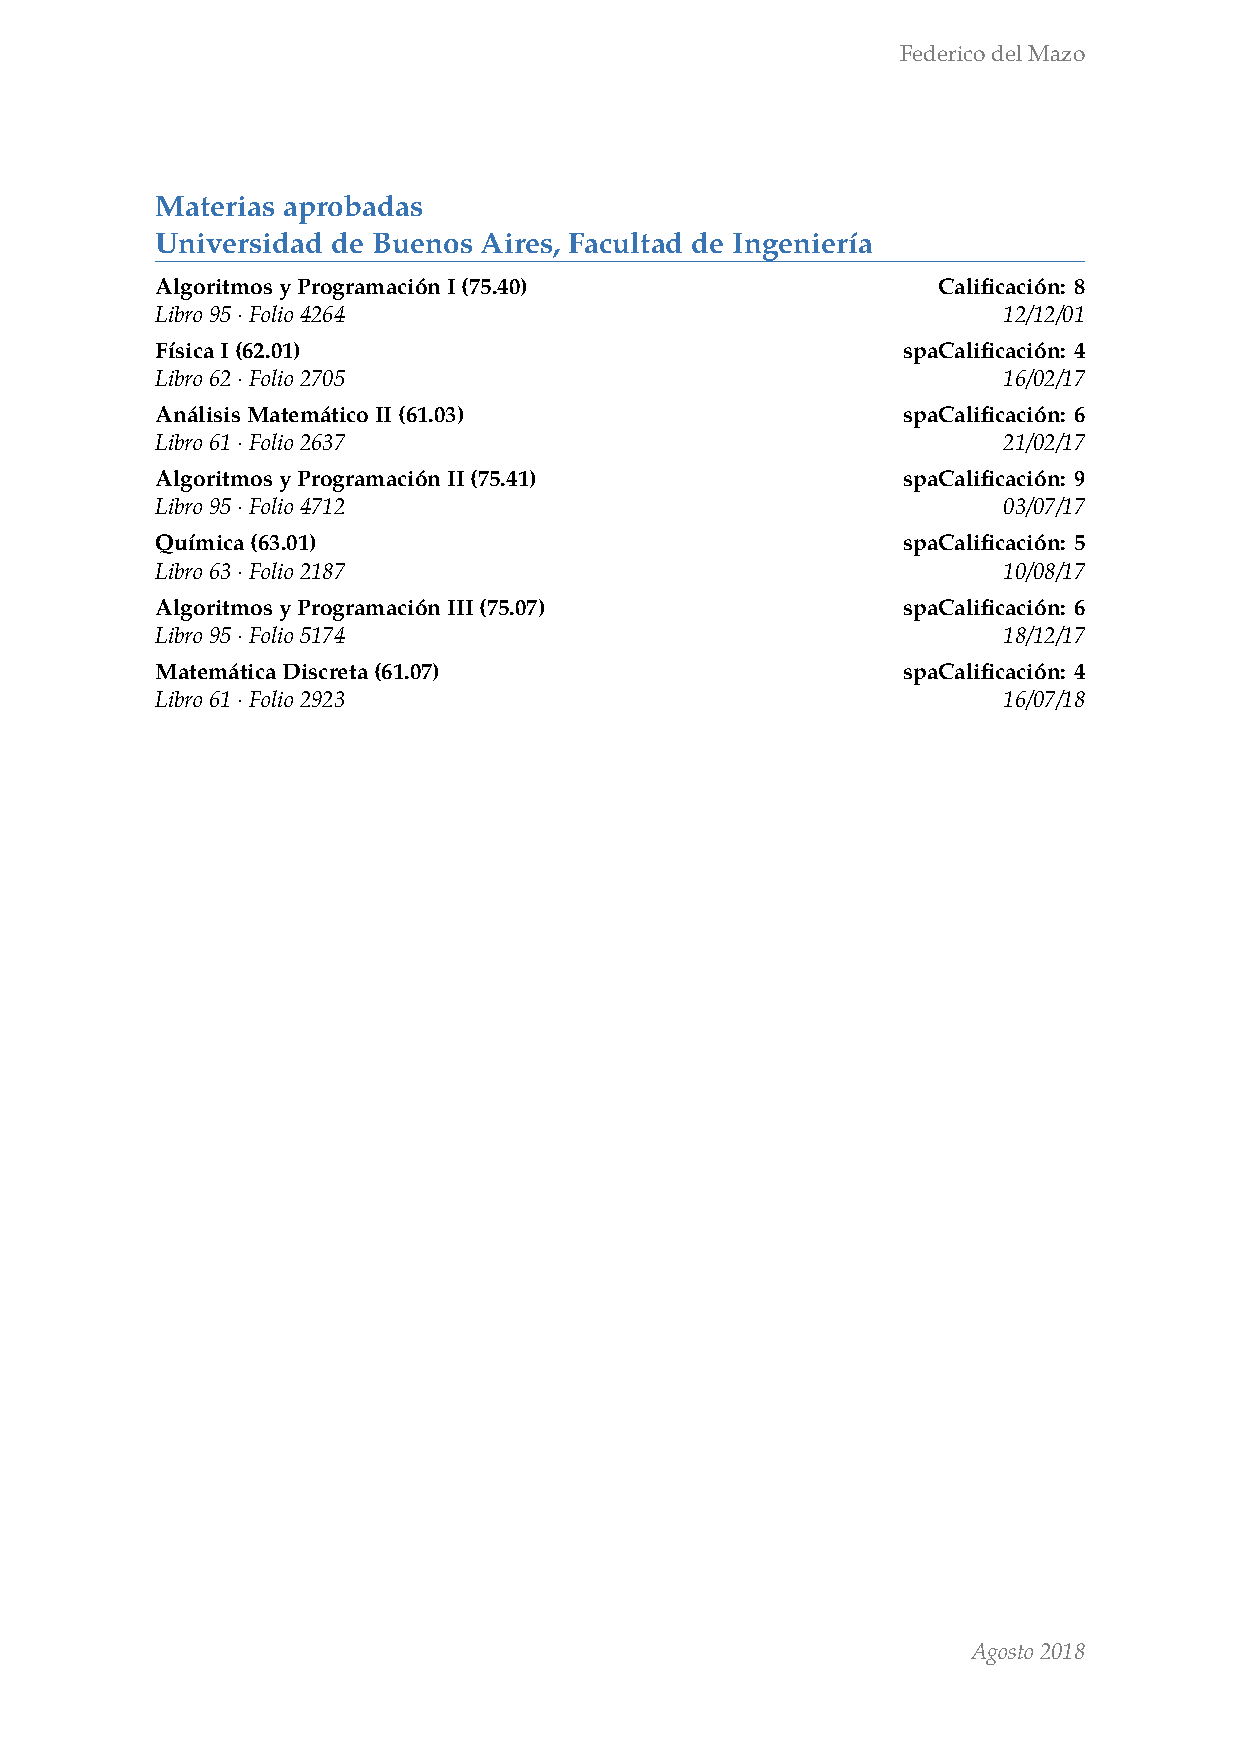
\includepdf[pages=-]{notas.pdf}}{}
\end{document}
